
\section{Abstract}

\quad The dataset from the ninth round of the Yelp Dataset Challenge was analyzed to determine which of the listed attributes are the most indicative of business success, as indicated by average star rating. Additionally, large quantities of review text were analyzed for sentiment and keywords originating from narratives relating to trauma to identify reasons for poor customer reviews. Whether or not the business was open or permanently shuttered at the time a review was written proved to be one of the best indicators of business category, more so than either latitude or longitude. Regardless of business location, the majority of the reviews were positive in sentiment, which correlates well with the average star rating of the reviews (around 3.7 also irrespective of location). No universal recurring problems were identified within the corpus, but time-series data of keywords from reviews from businesses with over 1000 reviews provided a method to visualize potential problems with businesses in one of several categories: service, food, price, or other.

\section{Introduction/Motivation}

\quad Yelp.com allows users to create an account and post public reviews of businesses. Our goal was to analyze the extensive data provided by Yelp as part of the Yelp Dataset Challenge to gain further insight for business owners to develop a more satisfactory experience for their customers. Yelp has a large public dataset available on their website with information about users, businesses, and reviews.

\quad Our first objective was to determine if certain attributes are indicative of business success with respect to their average review rating (see Related Work, Reviews and Revenue). Decision trees and k-means clustering were employed to group businesses by attributes with the highest information gain or shortest distance in attribute space, respectively. Furthermore, sentiment analysis was used on the language present in the reviews and compared with the star reviews to provide more information on a business’s chances of success. Information about the current state of a business and likely future states could be provided to businesses to permit them to change their current practices and focus to increase their chances of success.

\quad Another way sentiment analysis proved helpful in this project was to analyze the emotions conveyed by the reviewer as being pleased or angry at their experience with the business. Using the results of this analysis, our goal was to determine how certain times of day, city locations, or other factors contribute to customer experience. This information could also contribute to a business model. As an example, if certain locations are more prone to angry customers, it could indicate that the people in that area have high standards, the businesses are poorly run, or just that those customers tend to leave angry reviews. This type of information will be less useful to businesses, but it could prove very helpful for customers or advertisers to know that businesses in a certain area tend to be reviewed much higher or lower than the average business in cities of a comparable size. Also, to take an example, businesses reading their reviews on Yelp would be aware that the reviews in the area tend to be more negative than is average for the state, which in turn would prevent them from trying to fix problems that don’t exist.

\quad Our last objective was to find recurring problems in businesses. With natural language processing tools like NLTK, we analyzed review text to find the specific issues that people are having with businesses via keywords and repeated references to specific aspects of the business. If one of these businesses has many reviews which all indicate a similar issue, then that is useful information that a business owner would want to be aware of so that they can eliminate the problem, if possible. This was applied to reviews for businesses with a review count above a threshold, since businesses with few reviews are not likely to have enough information to examine recurring problems.

% Head 1
\section{Related Work}

\quad Since our project involves predictions surrounding businesses, we sought out similar research to guide our investigation. Thus, we focused our literature review on studies that utilized some form of sentiment analysis, constructed predictive models, and/or conducted meta-analysis of trends in the aforementioned sentiment, rating, or business interest.

% Head 2
\subsection{Predicting Business Attention}

\quad A previous winner, Hood et al. (2013), published a paper on assessing a business’s current rating/review state and future expectations with respect to review numbers on Yelp. The bulk of their work centered around the creation of additional features for the data (e.g., the number of similar businesses within 1 km, features of subsets of reviews such as average rating and number of unique users, etc.). From there they utilized various feature reduction and clustering techniques to build a prediction model. They were able to identify features that offered greater accuracy in prediction of interest in the business (calculated as the predicted number of reviews within 6 months after a target date) as well as create a model for prediction that outperformed a basic linear regression. Our approach was similar in the application of feature reduction to reduce data dimensionality, and the use of clustering to not only find cities with many businesses, but also group similar businesses together. However, save for the total_compliments feature created to help analyze the user data, we did not add additional features to the dataset like the number of nearby similar businesses.

% Head 3
\subsection{Latent Subtopics}

\quad Huang et al. (2013) utilized probabilistic models to discover underlying subtopics within Yelp reviews. This offered a framework to categorize the reviews based on review text. From here, they were able to analyze the prevalence of various star ratings within each category. In this way, they could advise business owners as to the common trends among good and bad reviews that may not be apparent without considering the review text. McAuley and Leskovec built on this idea by combining such latent review topics with hidden rating driving factors, allowing them construct a rating prediction model.

\subsection{Reviews and Revenue}

\quad In one of the more influential papers on the subject, Michael Luca showed a correlation between Yelp rating and revenue, highlighting the fact that rounding to half stars could significantly impact two similarly-rated restaurants if their averages fell on either side of the divide (e.g. 3.24 and 3.26). He goes on to build a model of market response based on review volume as well as the impact of user expertise. He concluded that such responses are consistent with a Bayesian learning model.

\subsection{Narratives and Consumer Sentiment}

\quad In an analysis of customer narratives embedded in Yelp reviews of restaurants in seven cities, Jurafsky et al. (2014) determined that negative reviews are likely to incorporate words and other features previously associated with trauma. Specifically, the incidence of words and phrases with a negative emotional slant, words relating to actions performed by third-person actors like waiters or management, and first-person plural pronouns like “we” and “us” is higher for negative reviews than positive. Meanwhile, positive reviews were characterized by language associated with addiction and, in the case of more expensive restaurants, sensory pleasure.

\quad To determine precisely which words were statistically overrepresented in the category of negative reviews, in this case taken to be reviews with one star, the authors applied a “log-odds-ratio informative Dirichlet prior” (originally published in Monroe et al. (2008)) to compare the frequency of each word in the full corpus to its frequency in the category of one-star reviews. The authors then sorted all the words by their log-odds association score to determine the 50 words that were most associated with one-star reviews. Rather than repeat their work, our group used a number of these words as given in the paper to determine the “issue distribution” of a particular restaurant over time (see Key Results, Tracking Problems).

\section{Dataset Information}

\quad The Yelp dataset comes from the Yelp Dataset Challenge. This is an ongoing challenge and this is the ninth round, so the challenge is very well-established by this point. The challenge offers \$5,000 to the winner and the final submission takes the form of an academic paper.

\quad We considered the following from the Yelp dataset:

\begin{itemize}
	\item{4.1 million reviews}
	\begin{verbatim}
	"review_id":(encrypted review id),
	"user_id":(encrypted user id),
	"business_id":(encrypted business id)"
	"stars":(star rating, rounded to half-stars),
	"date":(date, formatted: YYYY-MM-DD),
	"text":"review text",
	"useful":('useful' vote count),
	"funny":('funny' vote count),
	"cool": ('cool' vote count),
	"type": "review"
	\end{verbatim}
	\item{Information on 144,000 businesses in 11 cities from 4 countries (incl. the US, Germany, Canada, and the U.K. (with 1.1 million business attributes)}
	\begin{verbatim}
	"business_id":(encrypted business id),
	"name":"business name",
	"neighborhood": "hood name",
	"address":"full address",
	"city":"city",
	"state":"state"(if applicable),
	"postal code":"postal code",
	"latitude":latitude,
	"longitude":longitude,
	"stars":(star rating, rounded to half-stars),
	"review_count":(number of reviews),
	"is_open":0/1 (closed/open),
	"attributes":[(localized attribute tags)],
	"categories":[(localized category names)],
	"hours":[(hours strings)],
	"type": "business"
	\end{verbatim}
	\item{Over 1M users}
	\begin{verbatim}
	"user_id":(encrypted user id),
	"name":"first name",
	"review_count":(number of reviews),
	"yelping_since": (date, formatted: YYYY-MM-DD),
	"friends":[(encrypted user ids)],
	"useful":('useful' vote count sent by user),
	"funny":('funny' vote count sent by user),
	"cool": ('cool' vote count sent by user),
	"fans":"number of fans the user has",
	"elite":["an array of years the user was elite"],
	"average_stars":floating point average like 4.31,
	"compliment_type": (compliment count),
		...(same for each complement type)...
	"type":"user"
	\end{verbatim}
	\item{Over 200,000 user-submitted photographs, 947,000 tips, and aggregated check-in data for most businesses}
\end{itemize}

\section{Main Techniques}

\subsection{Data Cleaning and Preprocessing}

\quad Although the Yelp dataset was well formatted, its content was inconsistent. A lot of data was absent for nearly every attribute. Only a few attributes are guaranteed to exist for every business such as latitude and longitude. Businesses also contained an attributes attribute that had miscellaneous information about businesses; some examples of fields in attributes are Free Wifi, Garage Parking, etc. These are completely optional and are inconsistent among businesses. As a result of this inconsistency, we removed the attributes attribute from the dataset.

\quad The format of the data did not allow a successful import into Weka either in JSON or in CSV format, so instead we used RapidMiner, which incorporates extensive machine learning functionality like classification, regression, clustering, and association and frequent itemset mining. RapidMiner is commercial software, but an educational version is available that removes certain limitations on the free version like only being able to process 10,000 rows at a time. Additionally, RapidMiner was much more compatible with the missing data in our dataset and automatically corrects some of the formatting issues we had when attempting to use Weka. It does not support JSON so we reused the conversion code (found on the team GitHub as convert.py) to convert the data files to CSV.

\quad The remaining missing data from other attributes such as categories or address were more rare than the attributes attribute. Instead of removing the attribute completely, they were autocompleted with default values if certain data values were non-existent. For example, the categories attribute would be set a default value of null if a business lacks a category. These cases are rare at between 200 and 300 per attribute which is small compared to the 144,000 businesses.

\quad In other cases only the subset of attributes were used to determine clusters using k-means. This because k-means fails to work on non-numerical values. So attributes such as address or name was completely avoided. In the case of k-means the attributes used were latitude, longitude, review count, and stars. These were the only numerical attributes that was provided in the businesses dataset.

\subsection{Decision Trees and K-means Clustering}

\quad The decision tree was used on the Yelp dataset to breakdown classification for the category of a business. The decision tree was used to help categorize businesses based on the existing categories attribute for each business. Using the categories section as a label helped create a decision tree which split mainly on the is_open, latitude, and longitude attribute. These attributes yielded the highest information gain. Since a decision tree requires a label, the categories section became most logical to classify a business. As a result the cleaning of the categories attribute was important because it required no missing values to successfully label all businesses.

\quad K-means clustering with k = 5 was also used to find clusters. In order to perform k-means it was necessary to have numeric attributes only. This would mean removing attributes like the address. In addition to this the dataset was also missing 67-166 values. Once again this is relatively low number so it was decided to fill in the missing values with the average of the appropriate columns.

\subsection{Correlation Calculations}

\quad In order to better understand the users of Yelp and draw more complete conclusions from our findings, we did a brief analysis on our user data. Each user has an average of the stars they give in their reviews and the number of different types of compliments they’ve received on their reviews. Users also have a number of fans. We first created a correlation matrix with RapidMiner in order to see the relationship between average stars and compliments. Following this a new feature was created called “total_compliments”, which was a summation of the compliments that a user has received. We then created a new correlation matrix to see what the overall relationship was between average stars and total compliments. Finally, we created another correlation matrix to examine the relationship between fans and total compliments. The correlation matrices were exported from RapidMiner to an image by first converting the matrix to an example data type using the ‘Converters’ extension and then writing that data to an excel file. The table can then be formatted in the excel file and exported to an image.

\subsection{Natural Language Processing}

\quad To investigate the linguistic characteristics of the review corpus, a good deal of preprocessing was necessary. At the beginning, all of the reviews were in one 3.46-GB file, which consistently crashed RapidMiner and necessitated the use of custom scripts focused on extracting and analyzing the information of interest. Since the review file was too large to open with RapidMiner, a different method of “joining” the business data and the review data was necessary. The script extract_businesses_many_reviews.py was used to locate businesses with more than 1000 reviews, and write the business names, IDs (a unique tag provided by Yelp), and other selected attributes like that business’s average star rating to a separate file. The number 1000 was chosen somewhat arbitrarily, but the following processing is the most informative for businesses with many reviews. There are 177 businesses with more than 1000 reviews in the dataset.

\quad The script save_reviews_to_business_files.py was used to save all reviews for all businesses in the commonly-reviewed list to separate files, such that each file, named <business_id>.json, contained all the reviews for the business with that business ID. This step was important in building the processing pipeline, but could easily be eliminated now that the pipeline has been developed, so reviews for a certain business could be identified while the script loops through the large review file and then processed without an extra “save” step in between.

\quad Once all reviews for a business were in one file, the script problems_over_time.py was used to analyze the reviews and graph the results. To accomplish this, each review in a <business_id>.json file with a star rating of 3 or fewer stars was tokenized, stemmed, and compared to the following list of words associated with traumatic narratives in Fig.4 on the left:

\begin{figure}[h]
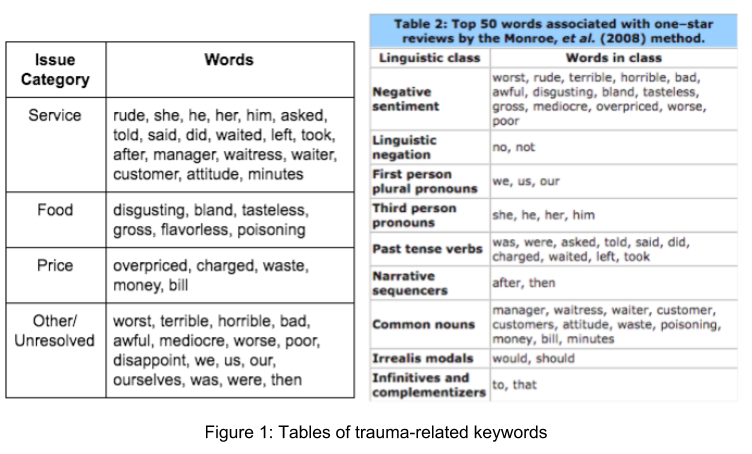
\includegraphics[width=0.75\textwidth, center]{table_trauma_keywords}
\end{figure}

\quad For comparison, the list of 50 words identified by Jurafsky et al. (2014) is on the right (see Related Work, Narratives and Consumer Sentiment). Notably, none of the seven cities used in the paper were among the set of cities provided by the Yelp Dataset Challenge, so there was a guaranteed overlap of zero reviews between the two corpora. Also, the list of words used for problem tracking over time was stemmed, eliminating the need to include plurals and different forms like “managers” as well as “manager,” or “waiting” and “wait” as well as “waited.” The count of stemmed forms of each of the words in the above left table was normalized by the total number of reviews for that month and graphed over time.

\section{Key Results}

\subsection{Basic Statistics and RapidMiner}

\quad After importing the CSV version of the data into RapidMiner, we tested some basic visualization tools included with the package. For instance, in Figure 1 we created a histogram of the average star for a business versus the state in which it is located. Basic graphs like these can help refine our questions. For example, why does Illinois have significantly lower average stars than other states or provinces, even those that border it?

\begin{figure}[h]
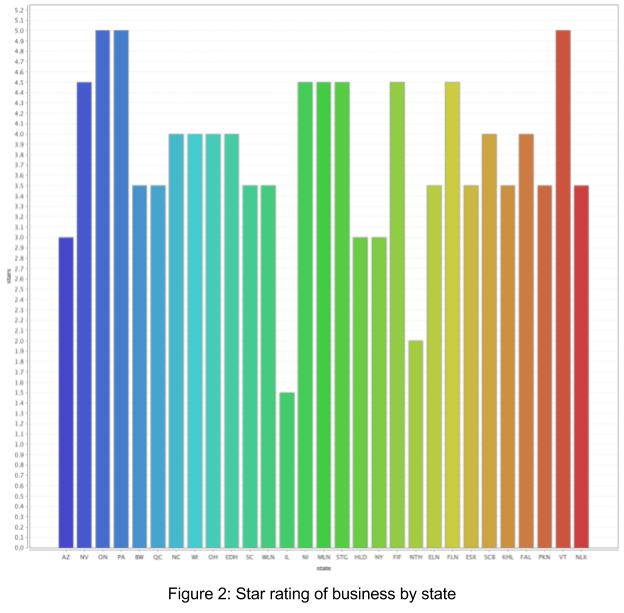
\includegraphics[width=0.75\textwidth, center]{b_rating_by_state}
\end{figure}

\quad RapidMiner can also produce 3D scatterplots which is useful because we used latitude and longitude in conjunction with the city and state to locate businesses, since some of the business address data is missing and cannot be filled with default values or other common values used to replace missing data. Figure 2 depicts a graph of longitude vs. latitude vs. review count for businesses.

\begin{figure}[!h]
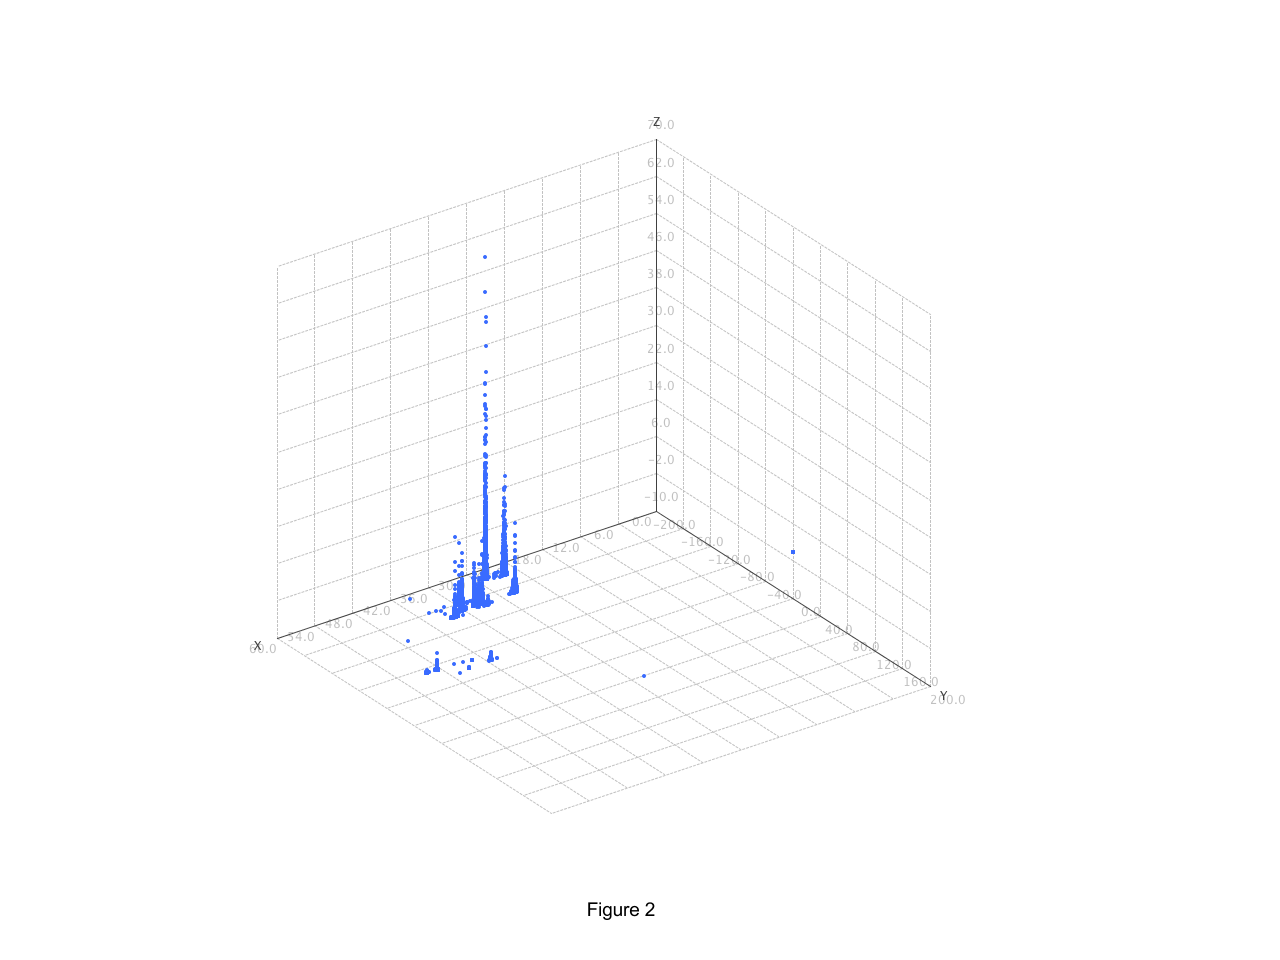
\includegraphics[width=0.75\textwidth, center]{3d_businesses_lat_long}
\end{figure}

\quad In this instance the visualization makes it clear that reviews are more frequent in populated cities as we expected. However, it also shows visually the outliers. There are various businesses that have only a few reviews. In this context it is easier to identify outliers and also see that businesses concentrate in certain locations, as is expected given Yelp?s declaration that the dataset focuses on businesses in 11 cities. Therefore we reduced the dataset to only the cities that meet the threshold of businesses or total review counts.

\subsection{Business Categories}

\quad In an effort to garner more information about user behavior, we needed to augment the initial data with that from the businesses and reviews, the latter of which serves as the link between the former two. In doing so, we attempted to profile the most frequent business reviewed by each user. The two troublesome business features were the user-defined ?tags? and ?categories?. The categories proved to be a more manageable problem as they are selected from a finite set of options. With numbers of selected categories ranging from two to 28 out of over 1000 possible choices, we sought to reduce this high degree of dimensionality.

\quad Sparse binary data of this kind quickly becomes unwieldy as traditional distance measures are highly prone to error. Such measures include k-Means, PCA analysis (for dimensionality reduction), DBSCAN, and agglomerative clustering. Typically, the computational cost is prohibitive (Plumpley, et. al. (2002)) or the numerical values are highly unstable during computation. The goal in our application is to reduce the effective categorical space and classify the businesses into a narrower subset?on the order of ~50. Not surprisingly, this scenario is almost identical to that encountered when processing and analyzing large corpuses of text. Almost every form of textual representation falls into the ?bag-of-words? paradigm where vectors are used to represent each document, and each element corresponds to either the frequency of a given term in the dictionary (i.e., all words from all documents) or the binary existence of the word in the document. Since each document is highly unlikely to have an instance of all terms, the combination of these vectors results in a very large, very sparse matrix of n documents by p terms.

\quad Much research has been done in recent years on Latent Semantic Analysis (or Indexing). This utilizes the fact that a given matrix?s Singular Value Decomposition provides us with a large degree of useful data concerning the nature of the matrix, namely which vectors and rows carry more weight as well as those with less impact. Furthermore, it provides a model through which new data can be projected onto the reduced subspace. The table below shows a sample of the reduced vector space and the first ten terms in each of the new topics.

\begin{figure}[!h]
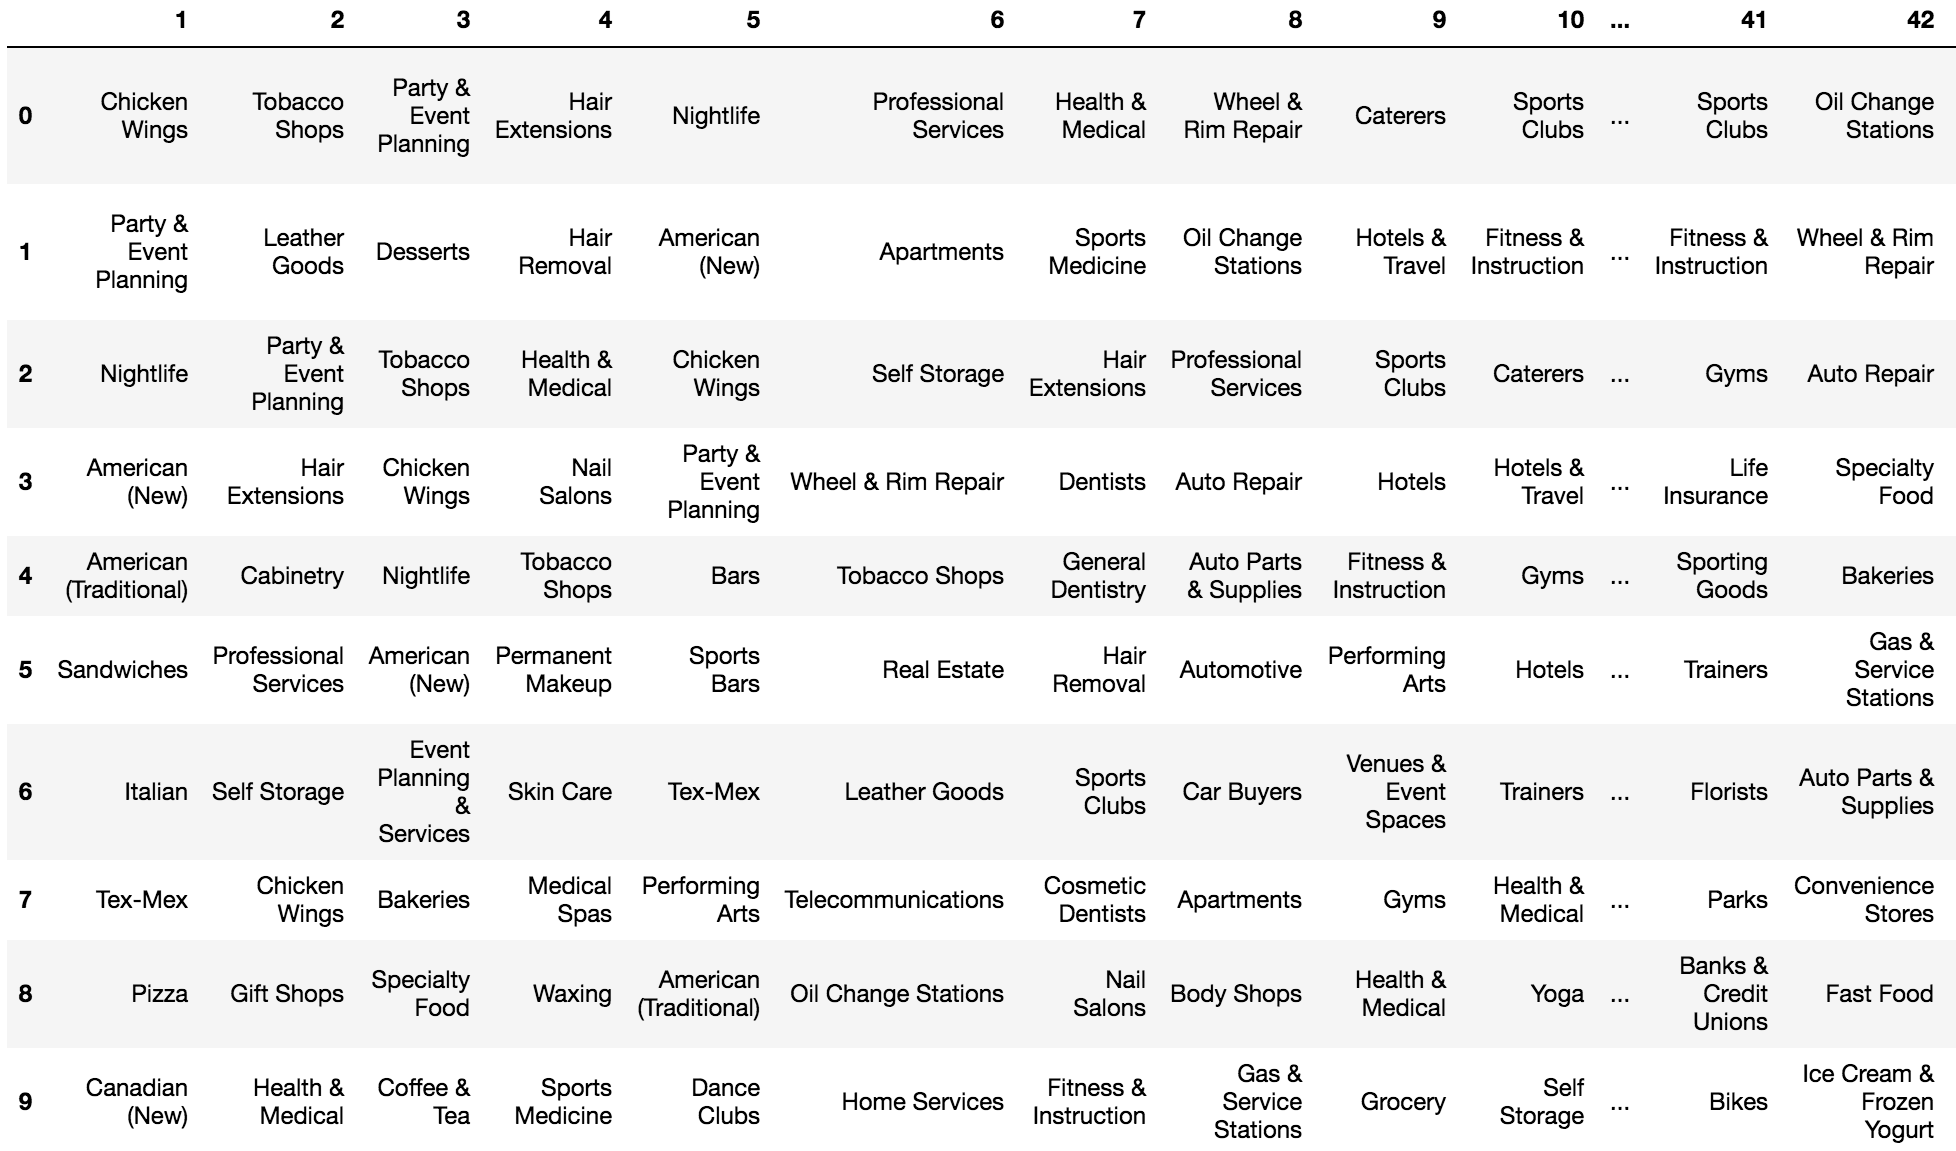
\includegraphics[width=0.75\textwidth, center]{topics}
\end{figure}

\subsection{Decision Trees}

\quad The decision tree shows the separation of businesses by categories. The tree provided insight into where the categories are dominant. As seen in Fig. 5 the tree breaks down into ranges of different latitude and longitude. The location of business has a strong correlation with the type of business. For instance in Fig. 5 the tree shows that a latitude of greater than 43.784 and a longitude of less than or equal to -73.477 yielded a large amount of categories. This is because this coordinate is in between New York City and Montreal which are high dense cities. The decision tree shows the best paths to take to determine the category of a business. The tree relies entirely on three attributes to determine a business’s category, is_open, latitude, and longitude. The location of a business is important so it is logical that a more dense variety of categories appear between Montreal and New York City as opposed to Arizona where there are fewer categories.

\quad The more interesting finding was that is_open is one of the main contributors to the category of a business. In retrospect the connection is clear because the failure of a business can have a domino effect. It is common to see a plaza or circle of businesses close down together because the location lacks popularity. Interestingly the tree prioritizes the is_open attribute higher than either the latitude or the longitude. If a business is open or closed permanently can actually determine the location and category of the business. One way of interpreting this is that it is very likely for a business to be a certain category if it is open or closed. The location is reflective of the trends and needs of that community. As a result many businesses of that type will either thrive or close in a certain latitude and longitude. Using the Montreal example before, the Canadian city has influence from New York City below it, the French, and of course Canadian culture itself. This blend of culture is well reflected in the culinary culture of Montreal. The tree in Fig. 5 portrays this area having categories of Food Delis, Comfort Food, Restaurants, Creperies, and Desserts. If a business is open and falls within those coordinates then it is likely that the business serves food of some sort.

\quad By contrast, the closed businesses tend to be more specialized and have an exact purpose within a certain community. Their locations are in less populated cities. For instance in Fig. 6, businesses that are categorized as Heating and Air Conditioning is in a less populated area. The color key below the node indicates the ratio of competing businesses in that same area. In the case of Heating and Air Conditioning it is the monopoly in its area. The business specializes in Heating and Air Conditioning where only a single type of this business is necessary in a smaller community. It is also follows that these locations are more obscure because they exist in areas where changes in weather are more extreme requiring the aid of this business.

\begin{figure}[h]
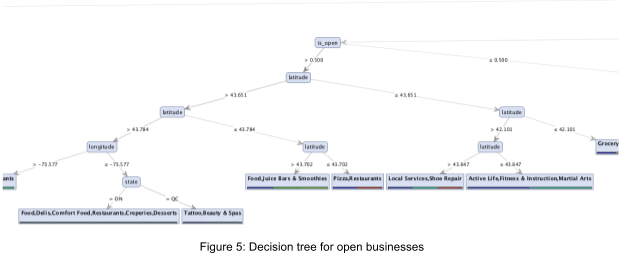
\includegraphics[width=0.75\textwidth, center]{decision_tree_open}
\end{figure}

\begin{figure}[h]
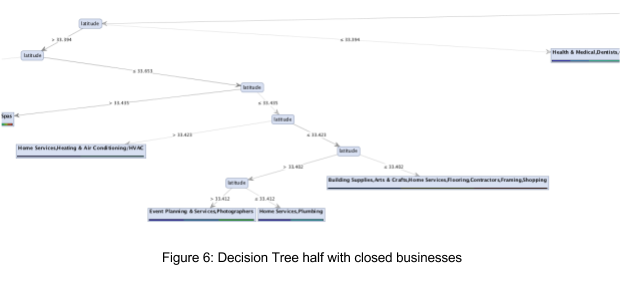
\includegraphics[width=0.75\textwidth, center]{decision_tree_closed}
\end{figure}

\quad The use of k-means returned results that were surprisingly consistent in star reviews (Fig. 7). Many of the businesses are in highly populated cities. As a result the k-means struggled to separate these businesses by location. However, k-means reveals the significant difference in average review counts by location. For instance the average review count for cluster 0 is ~207 reviews compared to cluster 1 which has ~18 reviews on average. However the average star rating is roughly similar around 3.7 stars. This pattern is seen in the other three clusters where differences in review counts still result in similar average star ratings. Across all clusters the stars are all near 3.7 stars average reviews. In cluster 2 the average star rating is ~3.5 which varies more significantly from the other clusters. The responding latitude and longitude is in the Massachusetts and New Hampshire area. The east coast has significantly less average review, but also lower star ratings as seen before. This may indicate more strict culinary culture on the east coast compared to the west with a relaxed comfort food culture. Yelp is a Silicon Valley company so its adoption and usage is likely more significant in western states.

\begin{figure}[h]
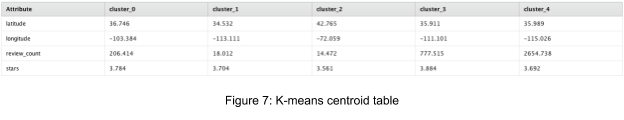
\includegraphics[width=0.75\textwidth, center]{k_means_centroids}
\end{figure}

\subsection{User Behavior}

\quad The users dataset essentially provides a window into users' status, connections, and interactions within the Yelp ecosystem. The figure below shows a plot of the user density versus the average star rating. We see that the density grows around 3.25-4.25 stars with some traces of a bell curve regarding the number of reviews the user has written.

\begin{figure}[!h]
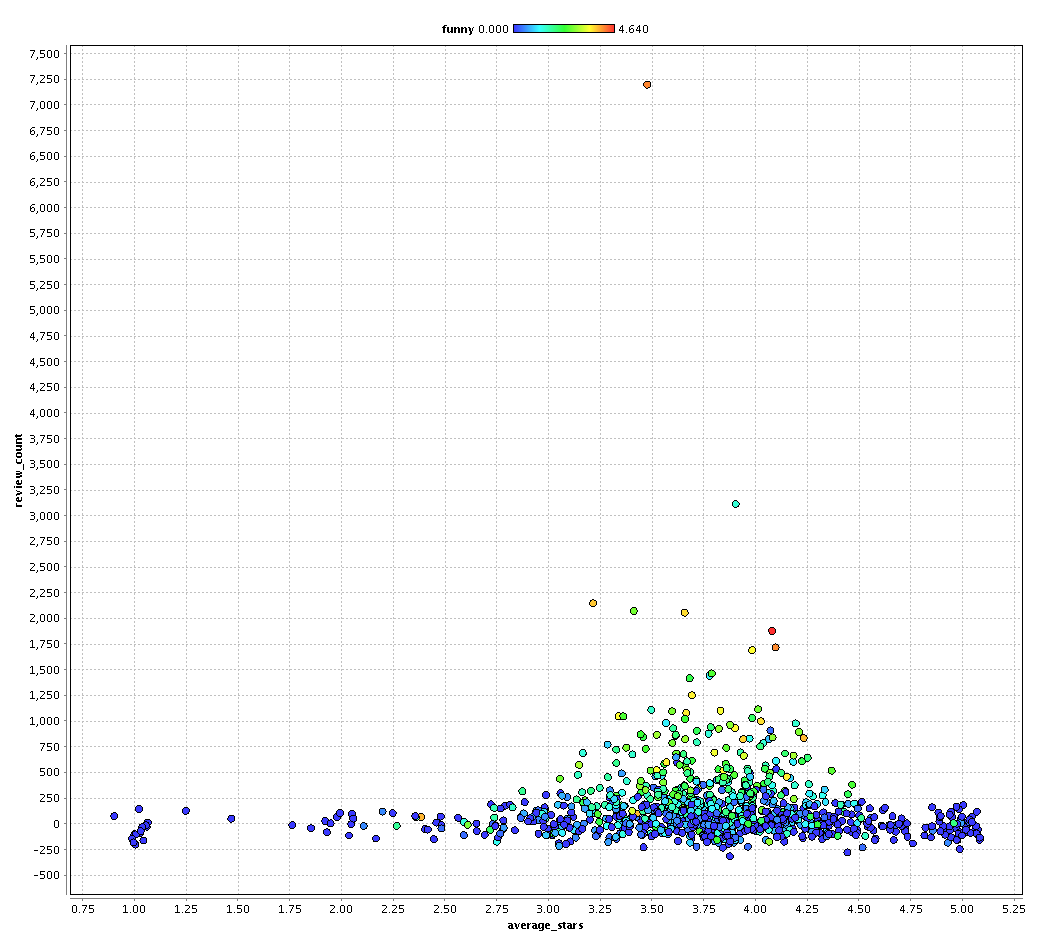
\includegraphics[width=0.45\textwidth, center]{u_reviews_vs_stars}
\end{figure}

\quad Our correlation matrices for the user data showed some insight into the social behavior on Yelp. Our first matrix included each complement type and the average stars a user gave in their reviews (Fig. 8). This matrix showed that there was not a correlation between the number of stars a user would give in their reviews and the compliments they receive. This seems to indicate that users would not be motivated to give a business a better or worse review in order to gain favorability in their profile.

\quad The second matrix (Fig. 9) includes the average stars feature and the total compliments feature. Again, there does not seem to be a relationship between star ratings given and the compliments received.

\begin{figure}[h]
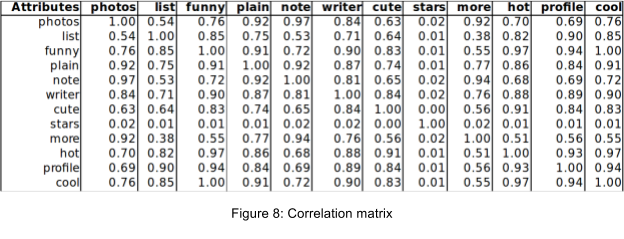
\includegraphics[width=0.75\textwidth, center]{correlation_matrix}
\end{figure}

\begin{figure}[h]
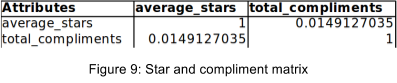
\includegraphics[width=0.75\textwidth, center]{star_and_compliment_matrix}
\end{figure}

\subsection{Tracking Problems}

\quad To answer the question of what types of problems were repeatedly present in a business, we built a utility that analyzes the language found in reviews. As mentioned in the Related Work section, Jurafsky et al. (2014) used a log-odds-ratio informative Dirichlet prior to determine the 50 words most statistically overrepresented in Yelp reviews with one star. We then used the stemmed forms of most of these words (see Fig. 4 in Main Techniques, Natural Language Processing) to determine the “issue distribution” for a particular business during a particular month, two examples of which are below as Fig. 10:

\begin{figure}[h]
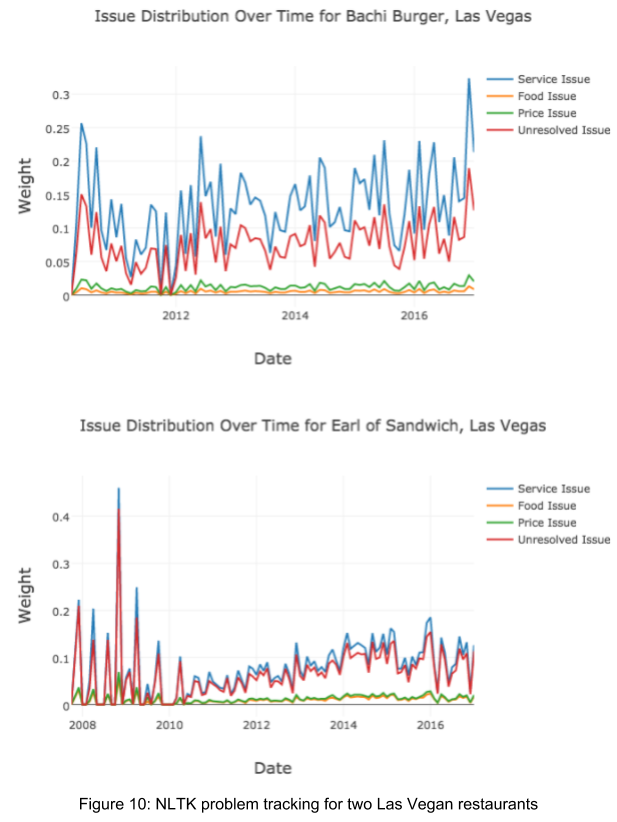
\includegraphics[width=0.75\textwidth, center]{nltk_tracking}
\end{figure}

\quad The high variability in weight seen in from 2008-2010 for Earl of Sandwich is due to a higher prevalence of negative words during every other month, which was a common occurrence in many of the analyzed restaurants. Restaurants were the only type of business from the review data that this analysis was applied to, because the “training set” of words provided by Jurafsky et al. (2014) were obtained from an analysis of restaurants. The spikes every other month could be the result of customers with high hopes visiting and coming away disappointed, leaving waves of more positive and more negative reviews. Additionally, it is worth noting that the average star rating for Bachi Burger within the dataset is 4.0, and the corresponding value for Earl of Sandwich is 4.5. Although both businesses had greater than 2700 reviews in the dataset, the number with 3 stars or fewer was substantially fewer, limiting the effectiveness of the analysis and providing another mechanism for the spikes seen in both graphs.

\section{Applications}

\quad The decision tree provides insight into the separation of businesses by their category. This can help classify the category of a new business or new areas. For instance, given a new business located at x latitude and y longitude, Yelp can make predictions based on surrounding categories. The tree also reveals the significance of a business being open or permanently closed, and potential declines in certain communities of businesses. Communities that have closing businesses are likely to have surrounding businesses close as well. In terms of businesses, this can help entrepreneurs choose areas that aren’t in decline when starting a new business.

\quad Latitude and longitude are also significant to the category of a business. For businesses this is important because certain categories become abundant in certain areas. One example is that in both New York City and Montreal there are a significant number of creperies because of New York City’s large population density and Montreal’s French influences. New businesses should consider other locations where creperies aren’t as popular. This can provide opportunities for new or existing businesses to venture into new areas. It can also help reveal the niche in certain communities such as in Fig. 4 where certain areas have relatively high concentrations of fitness-related businesses and even martial arts. New businesses can add to concentrations of businesses with an extra twist or bring quality to a category. This quality can be better determined with the k-means clusters.

\quad The clusters determined by k-means portray where Yelp is more impactful to a business. West coast areas receive more reviews on average. This can be helpful for businesses to measure their performance. Businesses that want to receive more feedback may consider the clusters that have higher review counts. It also reveals a more active community of Yelp which could be better business. There may be more competition in this clusters, but success can result in exponential growth in an active Yelp community.

\quad As mentioned in the introduction, the natural language processing performed on the review text to identify negative sentiment and recurring problems can be leveraged by managers and other staff members to improve their ratings, thereby improving revenue.


% Start of "Sample References" section

\section{Typical references in new ACM Reference Format}

A paginated journal article \citeA{Abril07}, an enumerated
journal article \citeA{Cohen07}, a reference to an entire issue \cite{JCohen96}, a monograph (whole book) \cite{Kosiur01}, a monograph/whole book in a series (see 2a in spec. document)
\cite{Harel79}, a divisible-book such as an anthology or compilation \cite{Editor00}
followed by the same example, however we only output the series if the volume number is given
\cite{Editor00a} (so Editor00a's series should NOT be present since it has no vol. no.),
a chapter in a divisible book \cite{Spector90}, a chapter in a divisible book
in a series \cite{Douglass98}, a multi-volume work as book \cite{Knuth97},
an article in a proceedings (of a conference, symposium, workshop for example)
(paginated proceedings article) \cite{Andler79}, a proceedings article
with all possible elements \cite{Smith10}, an example of an enumerated
proceedings article \cite{VanGundy07},
an informally published work \cite{Harel78}, a doctoral dissertation \cite{Clarkson85},

% Bibliography
\bibliographystyle{ACM-Reference-Format}{}
\bibliography{sample-bibliography}
